\begin{figure}
  \centering
  \begin{subfigure}{0.49\textwidth}
    \centering
    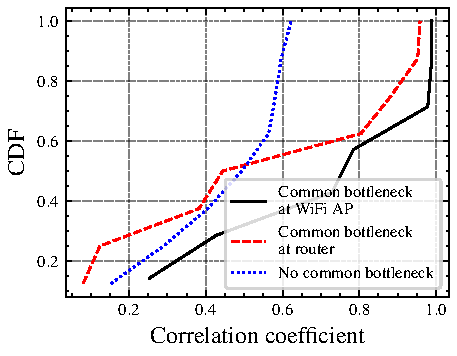
\includegraphics[width=\textwidth]{figures/bdp/bdp-05-no-video.pdf}
    \caption{\label{subfig:bdp-10}0.5 BDP}
  \end{subfigure}%
  \hfill
  \begin{subfigure}{0.49\textwidth}
    \centering
    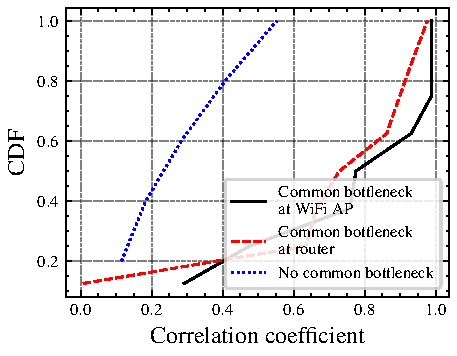
\includegraphics[width=\textwidth]{figures/bdp/bdp-10-no-video.pdf}
    \caption{\label{subfig:bdp-10}1 BDP}
  \end{subfigure}%
  % New line
  \vspace{1ex}
  \begin{subfigure}{0.49\textwidth}
    \centering
    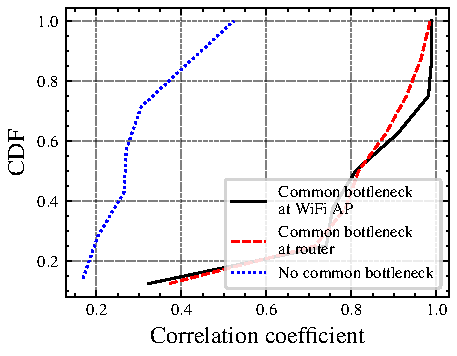
\includegraphics[width=\textwidth]{figures/bdp/bdp-15-no-video.pdf}
    \caption{\label{subfig:bdp-15}1.5 BDP}
  \end{subfigure}%
  \begin{subfigure}{0.49\textwidth}
    \centering
    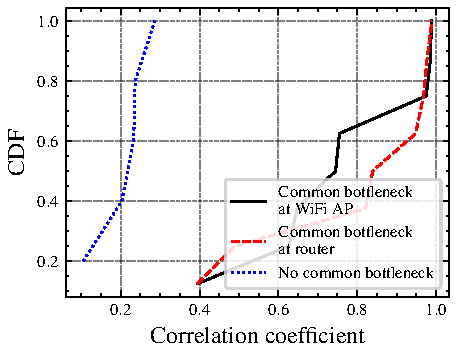
\includegraphics[width=\textwidth]{figures/bdp/bdp-20-no-video.pdf}
    \caption{\label{subfig:bdp-20}2 BDP}
  \end{subfigure}%
  %% \caption{\label{fig:cdf-bdp}CDF plots for each BDP configuration}
\end{figure}
